\documentclass[twocolumn]{article}
\setlength{\columnsep}{1cm}
\usepackage[utf8]{inputenc}
\usepackage{amsmath}
\usepackage{amsfonts}
\usepackage{amssymb}
\usepackage{hyperref}
\usepackage{listings}
\usepackage{appendix}
\usepackage{graphicx}
\graphicspath{ {graphs/} }

% \usepackage{listings}
\usepackage{color}

\definecolor{dkgreen}{rgb}{0,0.6,0}
\definecolor{gray}{rgb}{0.5,0.5,0.5}
\definecolor{mauve}{rgb}{0.58,0,0.82}

\lstset{frame=tb,
  language=Java,
  aboveskip=3mm,
  belowskip=3mm,
  showstringspaces=false,
  columns=flexible,
  basicstyle={\small\ttfamily},
  numbers=none,
  numberstyle=\tiny\color{gray},
  keywordstyle=\color{blue},
  commentstyle=\color{dkgreen},
  stringstyle=\color{mauve},
  breaklines=true,
  breakatwhitespace=true,
  tabsize=3
}

\newcommand{\hwname}{Jules Sang}
\newcommand{\hwemail}{jules.sang@grenoble-inp.org}
\renewcommand{\familydefault}{\sfdefault}

\title{Step 4}
\author{\hwname \\ \hwemail}

\begin{document}
\maketitle
\begin{abstract}
  In this paper I analyze the efficiency of different parsing algorithms.\\
  First part investigates on Chomsky normal form grammars with (i) a naive top-down algorithm, (ii) a memoization algorithm, and (iii) the widely-known CYK tabulation algorithm.\par
  Second part investigates on Linear grammars with (i) converting to Chomsky normal form then applying the CYK algorithm, (ii) directly adapting the CYK algorithm to linear grammars.\par
  Both parts give theorical and empirical views of the algorithms' efficiency.
\end{abstract}

\section*{Introduction}
Parsing is the process of analysing a string of symbols, conforming to the rules
of a formal gramar.
It is a fundamental computer science notion: The parser is one of the main
parts of compilers and interpreters, which describe how programs are executed by
the machine. Since most modern languages are context-free (and thus expressible
by context-free grammars \ref{cfg}), parsers for context-free languages can be
used to check that programs are syntactically correct.
% It is hence important to have the most efficient parsing algorithms.
Having efficient parsing algorithms hence allows a faster compilation or
interpretation of programs.

\section{Central notions}
\subsection{Context-free grammar (CFG)} \label{cfg}

% \href{https://en.wikipedia.org/wiki/Context-free_grammar}{Wikipedia} \\
% A context-free grammar is a grammar in which every production rule is of the form $A\rightarrow \alpha$, $A$ being a nonterminal symbol and $\alpha$ being a string of terminals and/or nonterminals. In a context-free grammar, the production rules can be applied on a nonterminal no matter which symbols surround it.

Parsers need set of formal rules in order to interpret the symbols of input
strings, and define a syntactic
relation between each other. This set of formal rules is called a grammar.
A context-free grammars is a special type of grammar. Context-free grammars can
express most modern programming languages.

\subsubsection{Definition}
A context-free grammar is defined by $G=(N,\Sigma,P,S)$, where:\\
\begin{enumerate}
  \item $N$ is a finite set, $n\in N$ is called a nonterminal element.
  \item $\Sigma$ is a finite set, $N\cup\Sigma=\emptyset$, $\sigma\in\Sigma$ is called a terminal element.
  \item $P:N\rightarrow (N\cup \Sigma)^*$ is a finite set of production rules.
    The ``*'' symbol expresses a multiplicity. Here it means ``any number of elements from
    $N$ and $\Sigma$''.
  \item $S\in N$ called the starting symbol of $G$.
\end{enumerate}
% $L(G)=\{w\in \Sigma^*|S\Rightarrow^*w\}$ (Where $S \Rightarrow^* w$ means that
% $w$ can be generated from $S$ by using one or multiple rules)
$L(G)=\{w\in \Sigma^*|w$ can be generated\footnote{Given a production rule
  $A\rightarrow \alpha$, we say that $A$ can generate $\alpha$.} with $S$ the starting symbol$\}$
is called the ``language'' generated by $G$, and corresponds to the set of
terminal strings that can be generated starting from $S$ with production rules
from $P$.

\paragraph{Example of CFG} 
\begin{align*}
  G&=(N,\Sigma,P,A)\\
  N&=\{A,B\}\\
  \Sigma&=\{\alpha,\beta\}\\
  P&=\{A\rightarrow\alpha B\beta | \alpha, B\rightarrow\beta A\alpha | \beta\}
\end{align*}

\subsection{Chomsky normal form (CNF)}
A context-free grammar $G$ is said to be in Chomsky normal form if all of its production rules are of the form
\begin{itemize}
\item $A\rightarrow BC$ or
\item $A\rightarrow\alpha$ or
\item $S\rightarrow\epsilon$
\end{itemize}
Where $A,B,C$ are nonterminals, $S$ is the start symbol, $\epsilon$ denotes the empty string. Also, neither $B$ or $C$ may be the start symbol. \\
Any CFG can be transformed into a CNF grammar, with a size no larger than the square of the initial grammar's size.

\subsection{Some common algorithmic techniques}
Here are the main idea of the algorithmic techniques used for this assignment.

\subsubsection{Tabulation}
Tabulation is a dynamic programming technique that focuses on building up larger and larger subsolutions to a problem until the target solution has been reached. Each iteration uses the results of the previous ones to compute the solution faster. Tabulation algorithm are bottom-up and iterative by nature.

\paragraph{Example of tabulation algorithm} Here is how one would use tabulation for computing fibonacci:\\
\begin{lstlisting}
  function fibo(n):
      mem[0] <- 0
      mem[1] <- 1

      for i in 2...n:
          mem[i] = mem[i-1] + mem[i-2]
      
      return mem[n]
\end{lstlisting}

\subsubsection{Memoization}
Memoization is a dynamic programming technique where the result of time-expansive function calls are stored in a data structure, in order to avoid recomputing them if the same inputs occur again. Memoization algorithm are top-own and recursive by nature.

\paragraph{Example of memoization algorithm} Here is how one would use memoization for computing fibonacci:\\
\begin{lstlisting}
  function fibo(n):
      if n < 2:
          return n

      if mem[n] is null:
          mem[n] = fibo(n-1) + fibo(n-2)
          
      return mem[n]
\end{lstlisting}

\subsection{Cocke-Younger-Kasami (CYK) algorithm}
The CYK algorithm is a parsing algorithm: The input is $G$, a context free grammar in CNF and $\alpha$ a string, and the output is true if and only iff $\alpha\in L(G)$, $L(G)$ being the language generated by $G$.\par
It is easy to tweak the algorithm so that it returns the rules of $G$ used for generating $\alpha$.

% \subsubsection{Main idea}
\subsubsection{Naive top-down implementation}
Let $G$ be the grammar, $\Sigma$ the set of nonterminals symbols of $G$, $P$ the rules of $G$, $\alpha$ the string to parse and $S\in \Sigma$ the starting symbol of $G$.\\
Here is how \textit{parse($S$, $\alpha$)} behaves:
\begin{itemize}
\item If $|\alpha|=1$: Return true if $(S\rightarrow\alpha)\in P$ else return false
\item If $|\alpha|>1$: For each $(S\rightarrow AB)\in P$, and for each possible partition of $\alpha$ into two parts $\beta$ and $\delta$, return true if
both \textit{parse($A$, $\beta$)} and \textit{parse($B$, $\delta$)} return true. If no such combination of $(A,B,\beta,\delta)$ is found, return false
% it is possible to parse both $\beta$ with $A$ as the starting symbol, and $\delta$ with $B$ as the starting symbol. If there is atleast one possibility, return true, else false.
\end{itemize}

This algorithm consists of a recursive enumeration of each rule applying possibility.

\begin{lstlisting}
    function naive(G: the grammar, S: the starting symbol, alpha[i, j]: the string):
        if j = 1:
            return G.contains(S -> alpha)

        for each P production rule of G, of the form S -> AB:
            for k = 0...j:
                if naive(G, A, alpha[i, k]) and naive(G, B, alpha[k, j]):
                    return true

        return false
\end{lstlisting}

% TODO: find the complexity
\paragraph{Complexity:}
The exact time cost is hard to compute, but we can get a worst case lower time bound which
will be sufficient for comparing this algorithm with the other ones:\\
Given an instance of size $n$, if we consider the two recursive calls of depth
$n-1$ (rooted in the instances $[1, n-1]$, and $[2, n]$), we get a recursion tree of height $n$ and of branching factor $2$. We can
hence express our lower bound as follows:\\
\begin{align*}
  T(n) &> n+2(n-1)|G|+4(n-2)|G|+\cdots +2^{n-1}|G|\\
  \Leftrightarrow T(n) &>|G|\displaystyle\sum_{i=0}^{n-1}2^i(n-i)\\
  \leftrightarrow T(n) &=\Omega(2^n)
\end{align*}

% I am not sure how to compute the complexity, even after Anna's hints, but practical experiments show that it is usually way worse than cubic. I would start with $T(n)=2T(\frac n2)|G|$
% Let $n=|\alpha|$. The Master theorem says the the cost of the function is $O(n^{log_2(n)})$. The cost hence explodes when the size of the string to parse gets bigger.\par
% In the next sections, we will see how dynamic programming can reduce the execution time.

\subsubsection{Top-down implementation with memoization}
The Top-down implementation of the CYK algorithm works just like the naive implementation but maintains a global three-dimensional boolean table $Z$.\\
Each time a recursive call such as ``\textit{parse($A$, $\alpha[i, j]$)}'' is made ($A$ being the starting symbol, and $\alpha$ the string to parse from index $i$ to $j$), the result is stored in $Z[A,i,j]$, so that if the result is needed again, it can be accessed in constant time.\\
That programming technique is called memoization and has the following characteristics:
\begin{itemize}
  \item It stops on the first positive result, instead of going through all of the possible subproblems, which can save time
  \item It has a recursive nature, which makes it easy to write but can cause excessive memory use with unadapted compilers
  \item It only requires a small adaptation of the naive top-down method, which is maintain and use the global table $Z$
\end{itemize}

\paragraph{Pseudocode} Here is the pseudocode for the top-down implementation:
\begin{lstlisting}
global Z
function TD(G: the grammar, S: the starting symbol, alpha[i, j]: the string):
    if j = 1:
        return G.contains(S -> alpha)

    for each P production rule of G, of the form S -> AB:
        for k = 0...j:
            if Z[A, i, k] is null:
                Z[A, i, k] <- TD(G, A, alpha[i, k]

            if Z[B, k, j] is null:
                Z[B, k, j] <- TD(G, B, alpha[k, j]

            if Z[A, i, k] and T[B, k, j]:
                return true

    return false
\end{lstlisting}

\paragraph{Complexity:}
At most, there will be as many recursive calls as there are cells in T, i.e. $|G|n^2$. Since the body of the function, except the recursive calls has a time complexity of $O(n)$, the total time complexity is $T(n)=O(n)*O(|G|n^2)=O(|G|n^3)=O(n^3)$

\subsubsection{Bottom-up implementation with tabulation}
Let $G$ be the grammar, $S$ the starting symbol, $\alpha$ the string to parse.\par

The following bottom-up implementation of the CYK algorithm is the original version that can be found in textbooks. The idea is to maintain a table of substrings that can be parsed by rules of the grammar, storing the possible starting symbol(s). The iterations start at substring size 1, and end at substring size $|\alpha|$. If $S$ is stored in the table for the size $|\alpha|$, $\alpha\in L(G)$. Note that previous iterations are used for building the next ones.\\
Let $P$ be the table of substrings. $P[a,b,c]$ is true iff the substring of $\alpha$ starting at index $c$ and of length $a$ can be parsed with the production rule of index $b$.\\
That programming technique is called tabulation and has the following characteristics:
\begin{itemize}
\item It has an iterative nature, which does not cause excessive memory use with any compiler, but it is usually harder to program
  \item It computes all of the possible problems, which can cost a bit of compututational time (without increasing the asymptotic complexity), but allows to give instantly the solution to any subproblem afterwards ($\displaystyle\bigcup_bP[a,b,c]\equiv parse(\alpha[c, c+a])$.
\end{itemize}

\paragraph{Pseudocode} Here is the pseudocode for the bottom-up implementation:
\begin{lstlisting}
function TD(G: the grammar, alpha[1, n]: the string):
    R[1, r] <- G.nonterminal_symbols // with R[1] the starting symbol of G
    let P[n, n, r] an array of boolean with all values initialized to false
    for s in 1...n:
        for each production rule R[v] -> a[s]:
            P[1, v, s] <- true
    
    for l in 2...n:
        for s in 1...n-l+1:
            for p in 1...l-1:
                for each production rule R[a] -> R[b]R[c]:
                    if P[p, s, b] and P[l-p, s+p, c]: 
                        P[l, s, a] <- true

    return P[n, 1, 1]
\end{lstlisting}

\paragraph{Complexity:}
Most of the work is done in four imbricated loops, three of them are bounded by $n$, and the last one
bounded by $|G|$.
We hence have $T(n)=O(n^3|G|)=O(n^3)$

\section{Empirical measurements}
Given the respective theorical complexities, we should expect a running time growing extremely fast as $n$ grows for the naive algorithm, and similar running times for the top-down and the bottom-up dynamic programming variants.
\subsection{Comparison with theoritical running time estimations}
\subsubsection{Well-balanced parentheses}
The grammar used for the next tests only accepts well balanced parentheses:
\begin{align*}
  S&\rightarrow SS | LA | LR\\
  A&\rightarrow SR\\
  L&\rightarrow (\\
  R&\rightarrow )
\end{align*}

% \paragraph{tests}\mbox{}\\
\textbf{$\frac n2$ opening followed by $\frac n2$ closing, i.e. (((...)))}\\
\textit{The naive complexity is too important for it to be on the graph.}\\
You may find the figure at appendix \ref{fig:plr}.
\\

\textbf{$\frac n2$ pairs, i.e. '()()...'}\\
You may find the figure at appendix \ref{fig:plr2}.
\\

Here, both the naive and the top-down variants show a linear complexity, whilst the bottom-up variant has a quadratic complexity. This probably comes from the fact that the bottom-up variant performs the parsing for every possible substring while the others algorithms stop at the first positive recursive call.\par
For the naive and the top-down DP algorithms, if the first recursive call (i.e. $k=0$) is positive each time, the cost is linear, since the recursion tree is equivalent to a basic for-each loop.\par
It is interesting to note that, in terms of effective computation time, the naive version is slightly faster, since there is no additional table management:\\
You may find the figure at appendix \ref{fig:plr3}.
\\

\textbf{closing parenthesis then $\frac n2-1$ pairs, i.e. ')()()...'}\\
\textit{The naive complexity is too important for it to be on the graph.}\\
You may find the figure at appendix \ref{fig:cplr}.
\\

\textbf{$\frac n2-1$ pairs, then opening parenthesis, i.e. '()()...('}\\
\textit{The naive complexity is too important for it to be on the graph.}\\
You may find the figure at appendix \ref{fig:plro}.
\\

\subsubsection{Stupid grammar}
The grammar used for the next tests does not generate any word ($L(G)=\emptyset$) but the parsing algorithms can still be applied on it. Here is how it looks:
\begin{align*}
  S&\rightarrow ST|TS\\
  T&\rightarrow a
\end{align*}
% \paragraph{tests}\mbox{}\\
\textbf{several a's, i.e. 'aa...'}\\
\textit{The naive complexity is too important for it to be on the graph.}\\
You may find the figure at appendix \ref{fig:as}.
\\

\section{Linear grammars}
\subsection{Turn it into Chomsky normal form}
This is the easy solution: Transform each rule that does not match CNF into CNF
rule:
\begin{align*}
  A\rightarrow B\alpha&\equiv A\rightarrow BC,C\rightarrow\alpha \\
  A\rightarrow\alpha B&\equiv A\rightarrow CB,C\rightarrow\alpha
\end{align*}
Since each initial rule generates at most 2 CNF ones, the size of the generated
CNF grammar is $O(2|G|)=O(|G|)$, $|G|$ being grammar's size. The transformation's time complexity is $O(|G|)$.

Since the CYK algorithm has a time complexity of $O(n^3|G|)$, and since $|G|$ can be considered unchanged after the transformation, the total parsing time complexity is $O(|G|)+O(n^3|G|)=O(n^3|G|)$.

\subsection{Adapting the CYK algorithm}
It is possible to adapt the CYK algorithm to parse linear grammars, changing the way the global three-dimensional table is updated. The idea is that instead of testing all the possible string partitions, we check partitions of size $(1, n-1)$ for rules of form $A\rightarrow\alpha B$ and partitions of size $(n-1,1)$ for rules of form $A\rightarrow B\alpha$.

Formally, the table is filled as follows:\\
Let $G=(N,\Sigma,P,S)$, $N$ being the nonterminal symbols, $\Sigma$ the terminal symbols, $P$ the production rules, and $S$ the starting symbol. let $t$ a global three-dimensional table, $s$ the parsed string and $n = |s|$.\\
$t[i,j]=\displaystyle\bigcup_{A\in N}\{A|A\rightarrow s[i]t[i-1,j+1]\in P\newline\lor A \rightarrow t[i-1,j]s[i+j-1] \in P\}$\\for $i\in [1,n],j \in [1, n-i+1]$\\
% TODO: explain that the first line is filled like with the CYK algorithm
If $S \in t[1,n]\quad s \in L(G)$, else $s \notin L(G)$.

Since the algorithm iterates over a $n^2$ sized array, and since the whole grammar is iterated for each cell, $T(n)=O(n^2|G|)<O(n^3|G|)$. It is hence worth it to adapt the CYK algorithm instead of turning $G$ into CNF.

\subsection{Empirical measurements}
It is interesting to compare the two precedent methods to verify that both follow the expected behavior.

\subsubsection{abc}
The grammar used for the next tests only accepts strings of form $a^kb^lc^k\ \forall k\in \mathbb{N}\ \forall l\in\mathbb{N}\backslash 0$:\\
\begin{align*}
  G&=(N,\Sigma,P,A)\\
  P&=\
  \left\{ \begin{array}{l}
    S\rightarrow Ac\\
    S\rightarrow b\\
    A\rightarrow aS\\
    A\rightarrow aB\\
    B\rightarrow bS
  \end{array}\right\}
\end{align*}

\textbf{Inputs from $L(G)$}\\
Here are the measured time complexities for strings from $L(G)$.\\
You may find the figure at appendix \ref{fig:complexity_as_bs_cs}.
\\

As expected, the adapted CYK algorithm's is $O(n^2|G|)$ for the given inputs, while turning $G$ into a CNF grammar is $O(n^3|G|)$.
\\

\textbf{Inputs not from $L(G)$}\\
Here are the measured time complexity for random strings not from $L(G)$, i.e. $\{\alpha=(a+b+c)^n|\alpha\notin L(G)\}$.\\
You may find the figure at appendix \ref{fig:complexity_random_abc}.
\\

With wrong inputs, The measured complexities preserves the same behavior. It is hence indeed more efficient to adapt the CYK algorithm.

\newpage
\onecolumn
\setcounter{section}{0}
\subsection*{Appendices}
% \appendix
% \appendixpage

\subsection{ }
\begin{center}
  \label{fig:plr}
  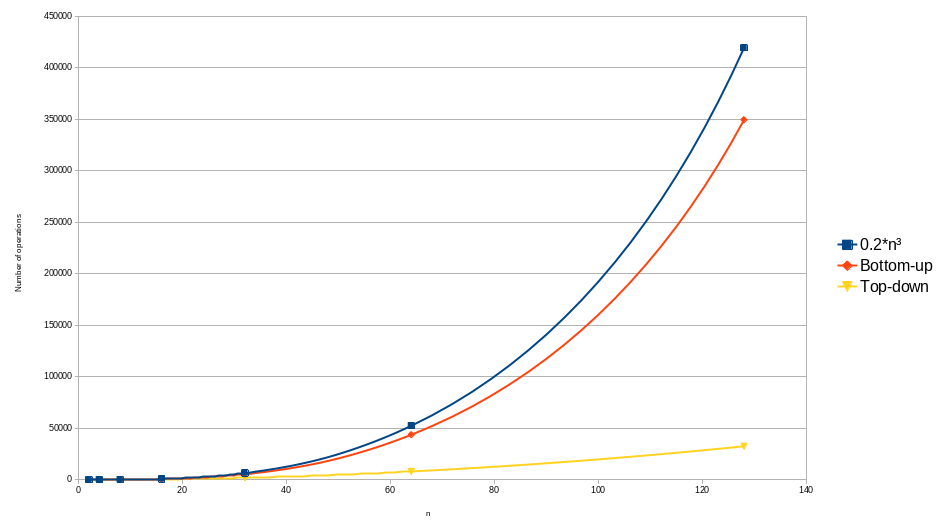
\includegraphics[width=\textwidth]{paren/complexity_paren_lefts_rights}
\end{center}

\newpage
\subsection{ }
\begin{center}
  \label{fig:plr2}
  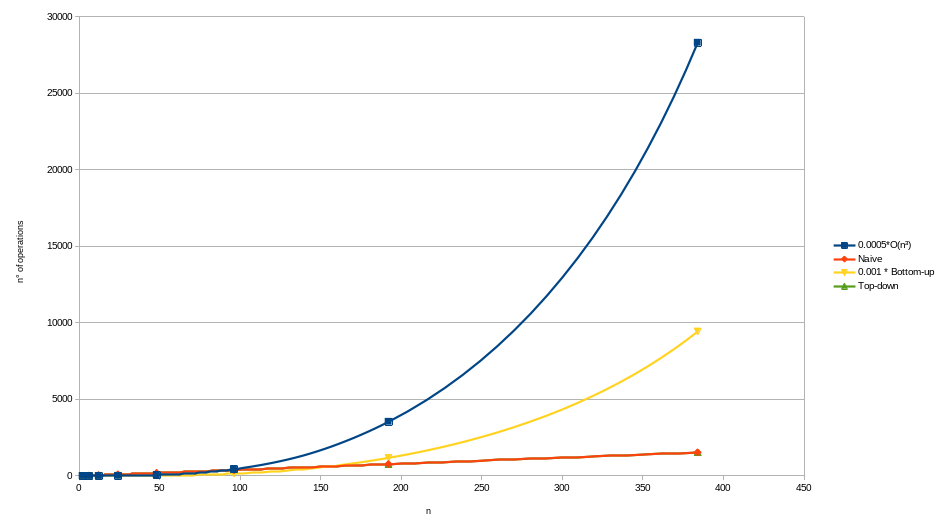
\includegraphics[width=\textwidth]{paren/complexity_paren_left_right}
\end{center}

\newpage
\subsection{ }
\begin{center}
  \label{fig:plr3}
  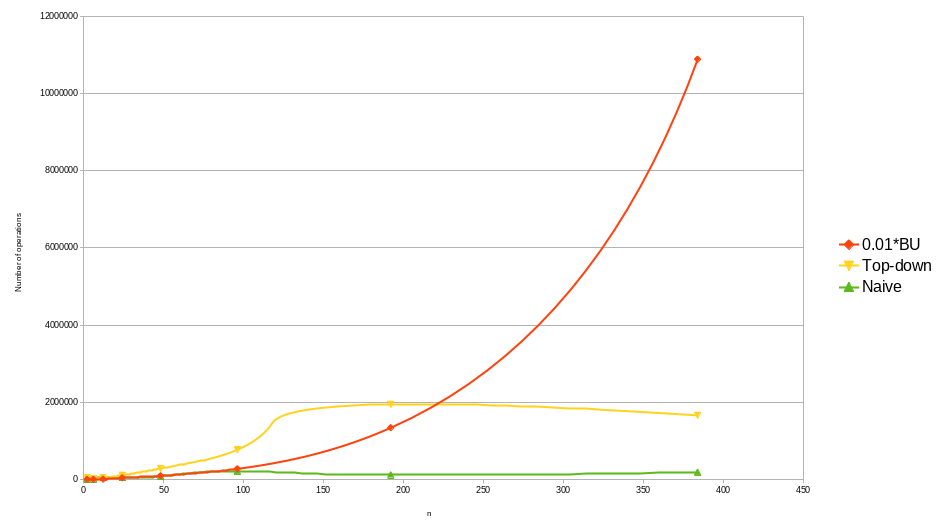
\includegraphics[width=\textwidth]{paren/time_paren_left_right}\\
\end{center}

\newpage
\subsection{ }
\begin{center}
  \label{fig:cplr}
  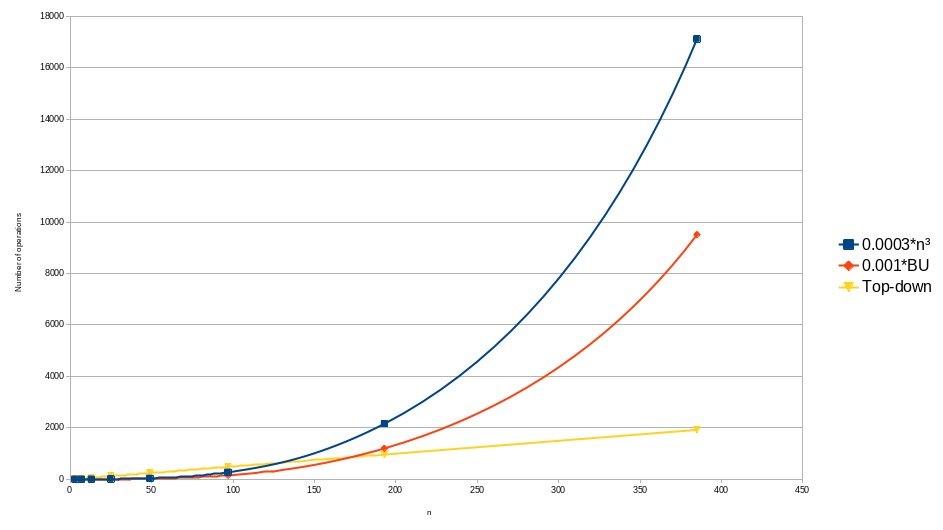
\includegraphics[width=\textwidth]{paren/complexity_closing_paren_left_right}
\end{center}
\newpage
\subsection{ }
\begin{center}
  \label{fig:plro}
  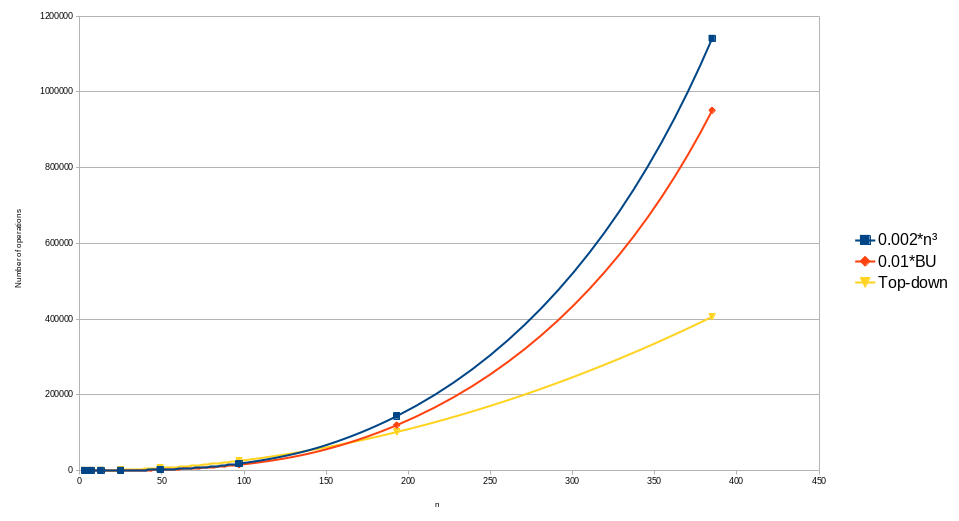
\includegraphics[width=\textwidth]{paren/complexity_paren_left_right_opening}
\end{center}
\newpage
\subsection{ }
\begin{center}
  \label{fig:as}
  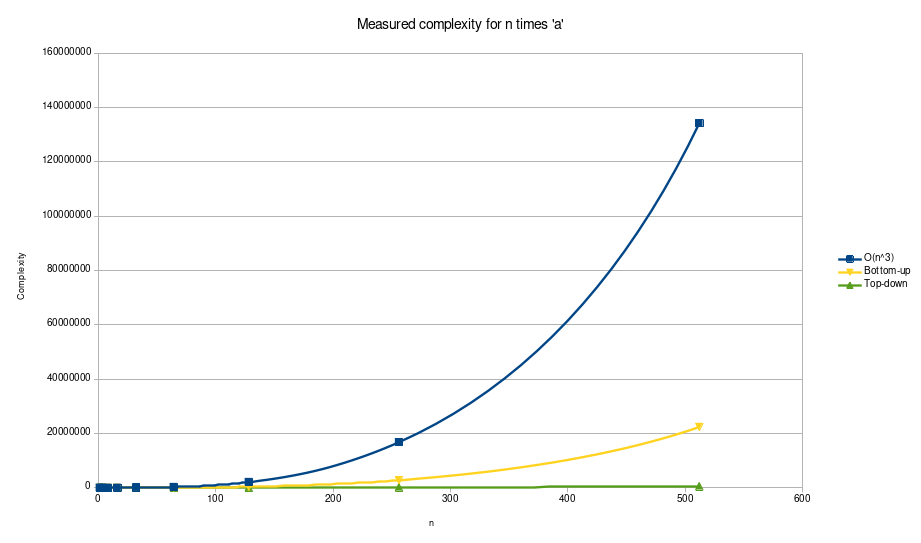
\includegraphics[width=\textwidth]{as/as}
\end{center}

\newpage
\subsection{ }
\begin{center}
  \label{fig:complexity_as_bs_cs}
  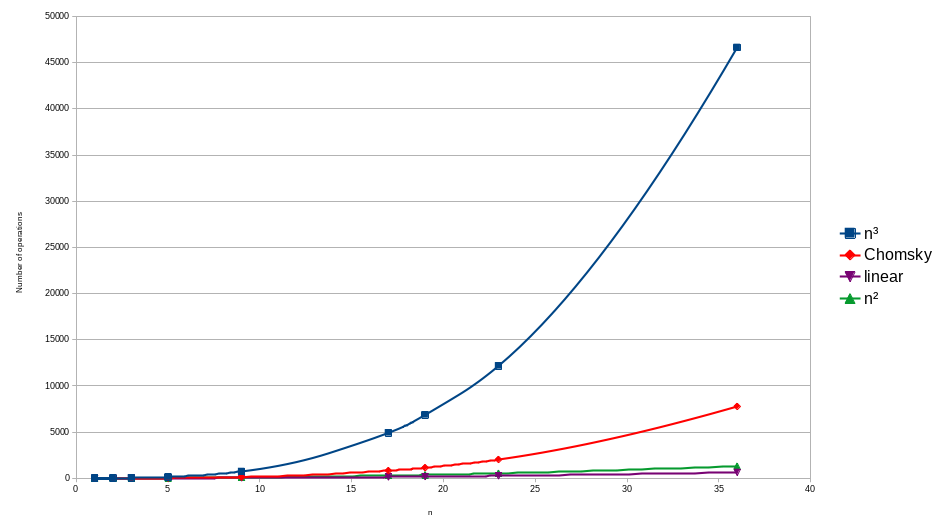
\includegraphics[width=\textwidth]{linear/complexity_as_bs_cs}
\end{center}

\newpage
\subsection{ }
\begin{center}
  \label{fig:complexity_random_abc}
  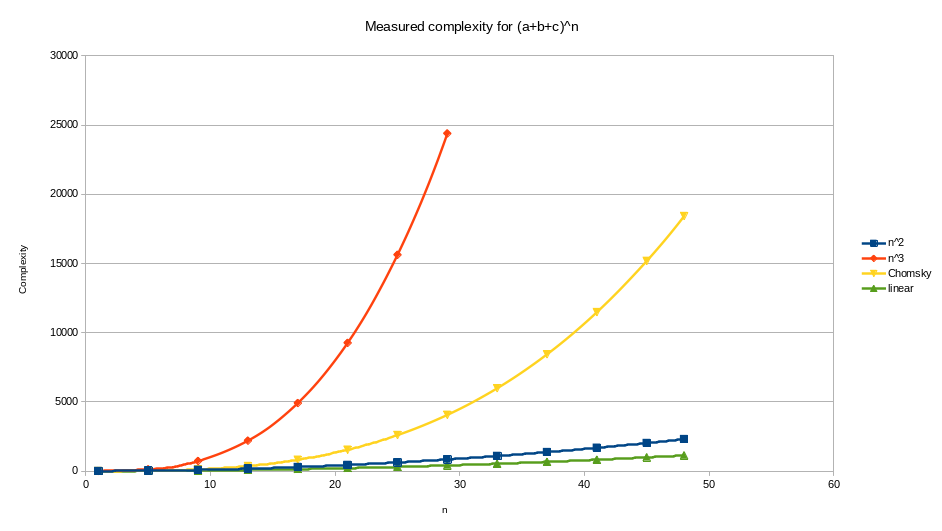
\includegraphics[width=\textwidth]{linear/complexity_random_abc}
\end{center}
\end{document}